\section{Sales}

There are two firms $i \in \{1,2\}$ and three customers $\{A, B, C\}$. The firms choose prices $\{p_1,p_2\}$ simultaneously. Customer A only wants to buy from firm 1 and has a value of $v$. Customer B only wants to buy from firm 2 and has a value of $v$. Customer C values both products at $v$ and buys from the cheapest firm (and flips a coin if the prices are the same). There are no costs so, assuming $p_i \leq v$, firm $i$'s profits are

\[
\pi_i = 
\begin{cases} 
p_i & \text{if } p_i > p_j \\
\frac{3}{2}p_i & \text{if } p_i = p_j \\
2p_i & \text{if } p_i < p_j 
\end{cases}
\]

%%%%%%%%%%%%%%%%%%%%%%%%%%%%%%%%%%%%%%%%%%%%%%%%%%%%%%%%%%%%%%%%%

\begin{tcolorbox}
    \begin{enumerate}
        \item[(a)] Argue there is no pure strategy Nash equilibrium.
    \end{enumerate}
\end{tcolorbox}

Let's assume that there exists a Nash equilibrium in pure strategies. In this case, the problem for each firm is to maximize its profit given the optimal strategy of the opposing firm:

\begin{equation*}
    \max_{p_i} \pi_i(p_i, p_j^*)
\end{equation*}

Where $p_j^*$ is the optimal strategy of the opposing firm. In the case of firm 1, it maximizes its profit when:

\begin{equation*}
    p_1^* = p_2^* - \epsilon_1, \quad \epsilon_1 > 0
\end{equation*}

We need to add the $\epsilon_1$ term to ensure that $p_1^* < p_2^*$, since otherwise the profit of firm 1 would be $3/2 p_1^*$, and, therefore, firm 1 wouldn't be maximizing its profit.

Similarly, firm 2 maximizes its profit when:

\begin{equation*}
    p_2^* = p_1^* - \epsilon_2, \quad \epsilon_2 > 0
\end{equation*}

Substituting $p_2^*$ into the equation for $p_1^*$ and vice versa, it is obtained that:

\begin{equation*}
    p_1^* = p_1^* - \epsilon_2 - \epsilon_1 \implies \epsilon_1 + \epsilon_2 = 0
\end{equation*}

\begin{myanswerbox}
    Which is a contradiction, since $\epsilon_1, \epsilon_2 > 0$ in order to maximize their profits. Therefore, there does not exist a Nash equilibrium in pure strategies.

    Intuitively, both firms must choose a price lower than the other in order to maximize their profits. This iterative decision-making process will lead to a simulated price war where both firms will end up choosing a price of zero. However, in this scenario, both firms have incentives to raise their prices to $\bar{p}$ to maximize their profits, even though they are not earning the maximum of $2\bar{p}$. At this point, the iterative process will restart, leading to the same conclusions.
\end{myanswerbox}

%%%%%%%%%%%%%%%%%%%%%%%%%%%%%%%%%%%%%%%%%%%%%%%%%%%%%%%%%%%%%%%%%

\begin{tcolorbox}
    \begin{enumerate}
        \item[(b)] We now derive the symmetric mixed strategy equilibrium. Suppose both firms choose random price with cdf $F(p)$ and support $[p,\bar{p}]$. Argue that $\bar{p} \leq v$. Write down firm 1's profit from price $p \in [p,\bar{p}]$.
    \end{enumerate}
\end{tcolorbox}

The profit function for firm 1, given the optimal strategy of firm 2, is:

\begin{equation*}
    \pi(p) = p (1 - F(p)) + p F(p)
\end{equation*}

Because $F(p)$ represents the probability to choose a price lower that $p$, and $1 - F(p)$ the probability to choose a price higher than $p$.

\begin{eqnarray*}
    \pi(p) &=& p (1 - F(p)) + 2pF(p)\\
    \pi(p) &=& p - pF(p) + 2pF(p)\\
    \pi(p) &=& p (1 + F(p))
\end{eqnarray*}

\begin{myanswerbox}
    So the profit function for firm 1 (and 2) in terms of the cdf $F(p)$ is:

    \begin{equation*}
        \pi(p) = p \left(1 +  F(p) \right)
    \end{equation*}

    Consumers only buy if the price is lower than their valuation, so the maximum price a company can charge is \( v \). If it charged more, consumers would not buy and the company would not make any profit. Therefore, \( \bar{p} \leq v \).
\end{myanswerbox}

%%%%%%%%%%%%%%%%%%%%%%%%%%%%%%%%%%%%%%%%%%%%%%%%%%%%%%%%%%%%%%%%%

\begin{tcolorbox}
    \begin{enumerate}
        \item[(c)] Argue that $\bar{p} = v$ in equilibrium.
        \item[(d)] Derive the distribution of prices $F(p)$ in equilibrium. What is the support of prices $[p, \bar{p}]$?
    \end{enumerate}
\end{tcolorbox}

In equilibrium, both firms should be indifferent between any combination of prices, including the case where both firms choose the same price. Therefore, the expected profit is:

\begin{eqnarray*}
    \pi(p) = p \left(1 +  F(p) \right) &=& \frac{3}{2} p\\
    1 +  F(p) &=& \frac{3}{2}\\
    F(p) &=& \frac{1}{2}\\
\end{eqnarray*}

This result states that the equilibrium price accumulates a mass of \( \frac{1}{2} \) at \( p \), a single point. This kind of distribution functions are from a family called Dirac delta functions, which are defined as:

\begin{equation*}
    \delta(x) = 
    \begin{cases}
        \infty & \text{if } x = p\\
        0 & \text{otherwise}
    \end{cases}
\end{equation*}

\begin{figure}[H]
    \centering
    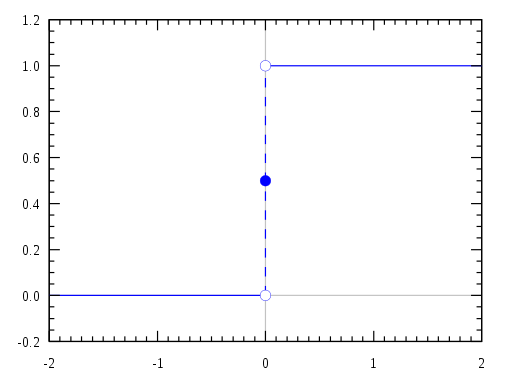
\includegraphics[width=0.5\linewidth]{plots/dirac-cdf.png}
    \caption{Dirac Delta CDF Centered in Zero}
    \label{fig:dirac-delta-cdf}
\end{figure}

\begin{figure}[H]
    \centering
    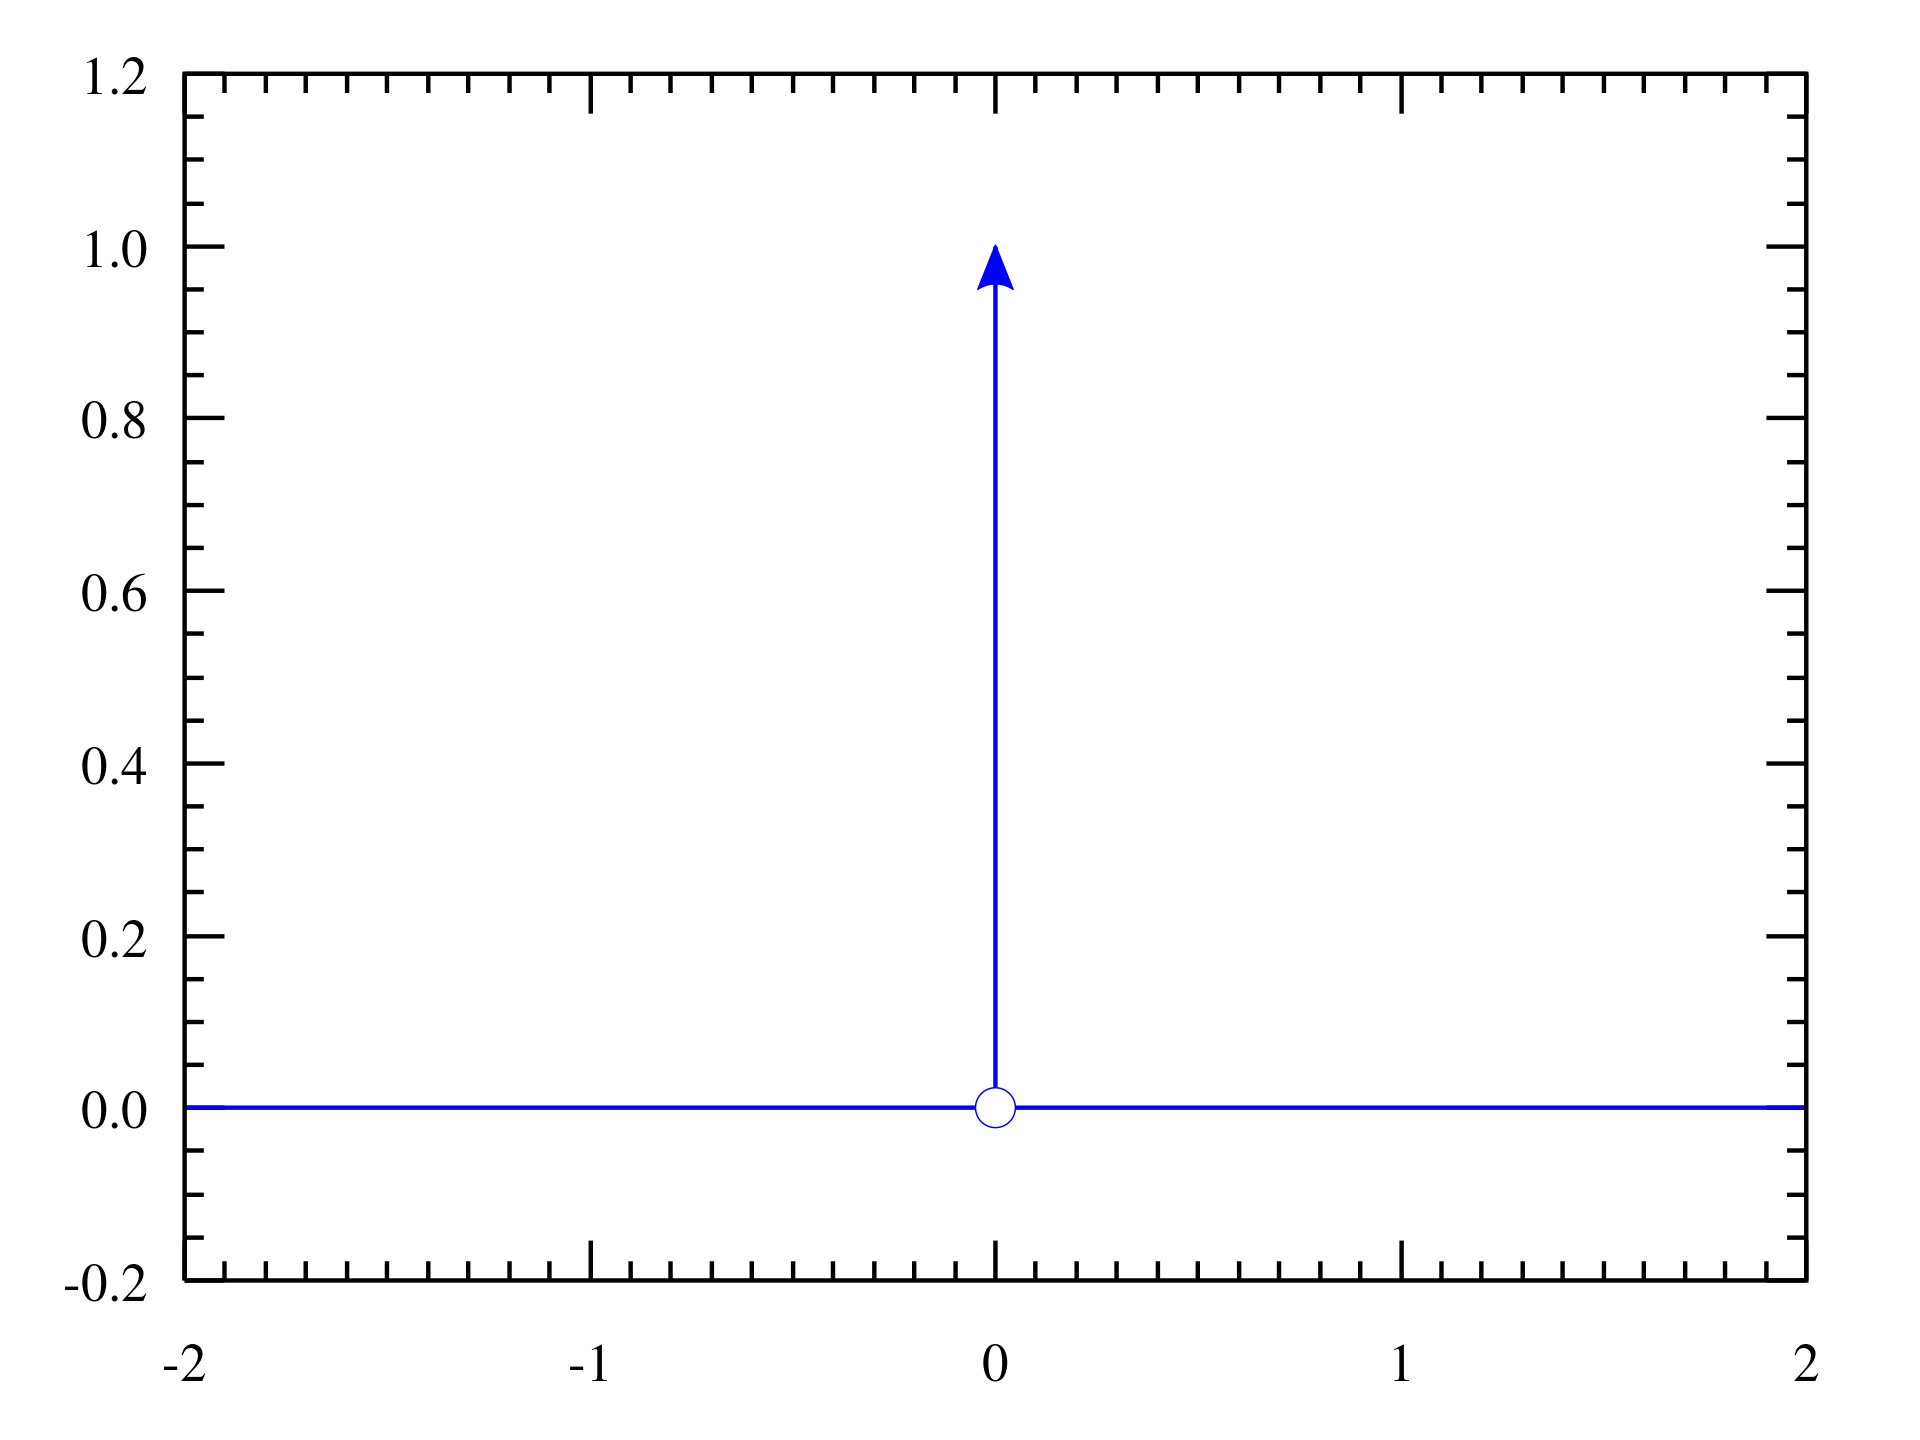
\includegraphics[width=0.5\linewidth]{plots/dirac-pdf.png}
    \caption{Dirac Delta PDF Centered in Zero}
    \label{fig:dirac-delta-pdf}
\end{figure}

\begin{myanswerbox}
    \textbf{Answer (c), (d)}:
    As we argued, the pdf of the equilibrium price follows a Dirac delta function centered in the equilibrium price. the function is defined as:
    
\begin{equation*}
    f(x) = 
    \begin{cases}
        \infty & \text{if } x = p\\
        0 & \text{otherwise}
    \end{cases}
\end{equation*}

\end{myanswerbox}

\begin{myanswerbox}
    As we explored in the previous questions, the equilibrium price should be lower or equal to the customer's valuation \( v \) in order to ensure at least one customer buys the product. Also, if the price is lower than \( v \), firms have incentives to start a price war with no equilibrium. Therefore, the equilibrium price is \( v \), and the support of the Dirac delta function is \([v, v]\), even though the function is defined for all real numbers.
\end{myanswerbox}
